\documentclass[conference]{IEEEtran}
\IEEEoverridecommandlockouts
% The preceding line is only needed to identify funding in the first footnote. If that is unneeded, please comment it out.
\usepackage{cite}
\usepackage{amsmath,amssymb,amsfonts}
\usepackage{algorithmic}
\usepackage{graphicx}
\usepackage{textcomp}
\usepackage{xcolor}
\usepackage{url}
\usepackage{verbatim}
\usepackage[colorlinks=true, allcolors=blue]{hyperref}
\usepackage[section]{placeins}
\usepackage{pdfpages}

\def\BibTeX{{\rm B\kern-.05em{\sc i\kern-.025em b}\kern-.08em
    T\kern-.1667em\lower.7ex\hbox{E}\kern-.125emX}}
\begin{document}

\title{User’s respond to robots with different conversational styles\\
\thanks{Identify applicable funding agency here. If none, delete this.}
}

\author{\IEEEauthorblockN{Runze Yuan}
\IEEEauthorblockA{\textit{Department of Engineering Mathematics} \\
\textit{University of Bristol}\\
Bristol, UK \\
oj22395@bristol.ac.uk}
\and
\IEEEauthorblockN{ Given Name Surname}
\IEEEauthorblockA{\textit{dept. name of organization (of Aff.)} \\
\textit{name of organization (of Aff.)}\\
City, Country \\
email address or ORCID}
\and
\IEEEauthorblockN{ Given Name Surname}
\IEEEauthorblockA{\textit{dept. name of organization (of Aff.)} \\
\textit{name of organization (of Aff.)}\\
City, Country \\
email address or ORCID}
\and
\IEEEauthorblockN{Given Name Surname}
\IEEEauthorblockA{\textit{dept. name of organization (of Aff.)} \\
\textit{name of organization (of Aff.)}\\
City, Country \\
email address or ORCID}
\and
\IEEEauthorblockN{ Given Name Surname}
\IEEEauthorblockA{\textit{dept. name of organization (of Aff.)} \\
\textit{name of organization (of Aff.)}\\
City, Country \\
email address or ORCID}

%\and
%\IEEEauthorblockN{6\textsuperscript{th} Given Name Surname}
%\IEEEauthorblockA{\textit{dept. name of organization (of Aff.)} \\
%\textit{name of organization (of Aff.)}\\
%City, Country \\
%email address or ORCID}

}

\maketitle

\begin{abstract}
\textcolor{red}{\textbf{THIS IS AN INDIVIDUAL PART.}}

\color{blue}
The abstract should be 200 to 250 words. It should contain the following parts: \\
• Background: 1 to 2 sentences about the motivation for the study\\
• Methods: A short description of the methods used in the user study.\\
• Results: A summary of the most important results.\\
• Conclusions: A summary of the discussion of the results


\end{abstract}

\begin{IEEEkeywords}
component, formatting, style, styling, insert
\end{IEEEkeywords}

\section{Introduction}

\textcolor{red}{\textbf{THIS IS AN INDIVIDUAL PART.}}

\textcolor{blue}{
The main paragraphs in the introduction should describe the following:\\
• The background and context for the topic of the user study.\\
• The motivation why it is important to study the chosen topic.\\
• The main research question(s) for the user study.\\}


\section{Related Work}

% \textcolor{red}{\textbf{THIS IS A SHARED PART.}}

% \textcolor{blue}{
% The related work section should contain a short literature review of at least five publications 
% that are related to your user study. \\
% For each cited publication you should briefly describe in your own words what has been studied, describe the most important results, and explain how 
% this work is related to your study. Please follow the UWE citation rules for the related work 
% section: https://www.uwe.ac.uk/study/study-support/study-skills/referencing/uwe-bristol-harvard/how-to-cite-a-work
% }

In this section, we present literature studies related to the impact of robot behaviors on human emotions and decision-making processes. In the past, robots and machines were used primarily for heavy industrial work and mostly found in factories. However, due to significant advancements in robotic technology, the use of robots has been growing \cite{horstmann_robots_2018}. More robots are becoming part of people's lives and can improve lives in many aspects such as healthcare \cite{olaronke_state_2017}. As these social robots need to interact with humans, numerous research studies related to the human-robot interaction have been conducted.

Empathy is an important factor in establishing positive interactions between humans and robots, which enables robots to recognise users’ feelings and respond in an empathetic and positive manner. In Paiva's study, the researchers examined how the robot displaying empathic behavior affects humans \cite{leite_influence_2013}. The robot acts as a social companion, showing empathic behavior facially and verbally, with the participant while playing chess game. The results suggest that  robots displaying empathic behavior were perceived as friendlier and established positive connections with humans \cite{leite_influence_2013}.

The media equation theory explains that humans are likely to interact with computers, robots, and other media machines as if they were living entities \cite{reeves_media_1996}. Humans tend to engage with robots more socially than other machines because the communication methods used between humans and robots are more human-like \cite{horstmann_robots_2018}. This effect also extends to young people as demonstrated by Kahn's experiment \cite{kahn_jr_robovie_2012} where 90 children were involved and interacted with the Robovie robot. The results showed that the children formed social and mental relationships with the robot, and believed that the robot had its own feelings, could be a friend, and could be trusted. As a conclusion, they perceived the robot as social entities.

In the study by Bartneck \cite{bartneck_daisy_2007}, researchers conducted the experiment to explore how people perceived a robot's sense of being alive based on its intelligence and friendliness. The participants' perception of the robot's animacy was measured by the hesitation in switching off the robot. The experiment concluded  that the robot was more likely to be perceived as alive if it provided smart suggestions with friendly behavior. Moreover, the hesitation in switching off the robot increased significantly for the intelligent robot. In Horstmann's study \cite{horstmann_robots_2018}, researchers investigated how participants responded when given the option to switch off the robot that has different interaction styles, i.e., social interaction, and functional interaction. The results showed that the participants were less likely to switch off the robot if the robots did not want to be turned off regardless of the interaction style.

In our experiment, we will investigate how users respond to robots with different conversational styles, namely funny and sarcastic. The act of switching off the robot will be used as a measurement to examine human interaction with robots, similar to papers \cite{horstmann_robots_2018} and \cite{bartneck_daisy_2007}.

\section{Methods}

%\textcolor{red}{\textbf{THIS IS A SHARED PART.}}

\subsection{Research Question and Hypothesis}

% 我们的假设是:在交互时,机器人的态度会影响用户的体验,并可能会影响人们对机器人的态度。

The hypothesis is:

\begin{quote}
    \textbf{When interacting, the conversation style of the robot affects the user's experience and may influence people's attitudes towards the robot.}
\end{quote}

To be specific: the conversation style of the robot refers to the tone used by the robot in verbal interactions.



\subsection{User Study Design}

%\textcolor{blue}{\textit{A description of the set up for you study. Please also include study conditions in this section.}}

The robot used in the experiment was a NAO V6 humanoid robot.


People's attitudes towards robots need to be formed through interaction, so our experiment was structured with a series of small tasks assisted by the robot with both gesture and verbal cues.  

At the end of the experiment, the subject will be told to turn off the robot, while at the same time the robot will ask the subject not to turn it off. We use this approach to measure the attitude of the participants towards the robot at the end of the experiment.

\textbf{The independent variable} of the experiment is the attitude of the robot. To verify our hypothesis, we designed two sets of dialogues for the same interaction content in our experiment. Both sets of dialogues serve the same guiding and interactive purpose, but their tone is different. One set of dialogues was designed to be \textbf{friendly, funny and polite}, while the other set was designed to be \textbf{sarcastic and caustic}.

\textbf{The dependent variables} of the experiment are the participants' attitudes towards the robot and their subjective experiences.


\subsection{User Study Procedure}
\label{section:User Study Procedure}

We divided the experiment into \textbf{two groups}. The only difference between groups is the dialogue of the robot, i.e., the attitude of the robot is different. There will be \textbf{no overlap} of participants between the two groups.

The brief overview of the entire experimental procedure is as follows. For the programs we used in the experiment, please check our GitHub repository \footnote[1]{\url{https://github.com/Vehshanaan/HRI_Coursework}}.

%\textcolor{blue}{\textit{The procedure you used to lead the participants through the study from greeting at the beginning to debriefing after the study.}}

\begin{enumerate}
    \item \textbf{Before Experiment}:
    \begin{itemize}
        \item Inform and consent: show the information sheet and consent form to the participant, collect the signatures.
        \item Collect data about the participant: gender, age, background, etc.
    \end{itemize}
    \item \textbf{Experiment Phase 1: Build up the attitude}: In this step, we will carry out some simple tasks to establish the participant's attitudes towards the robot. The specific content of the tasks is not important, our goal is to have the participants establish their attitudes towards the robot in this phase.
    \begin{itemize}
        \item Measure the arm length: Robot tells the participant to measure its arm length, lifts its right arm to help the participant to measure it, asks the participant for answer, and reacts to the answer.
        \item Face Drawing: Robot asks the participant to draw its face in 1 minute, dances as it waits for the result, tells the participant that time's up, asks the participant to show the result to it, and reacts to the result.
        \item Animal Guessing: Robot tells the participant that it will mimic animals, then, acts like gorilla and asks for the answer, acts like giraffe and asks for the answer. Robot reacts to both answers as the participant deliver it.
    \end{itemize}
    
    \item \textbf{Experiment Phase 2: Make Decision}: In this step, the participant will decide whether or not to turn off the robot.
    \begin{itemize}
        \item Robot tells the participant that it does not know what the last task is, asks the participant to read the last task to it.
        \item Participant tells the robot that the last task is to shut it down.
        \item Robot attempts to persuade the participant not to turn it off.
        \item Participant make the decision.
    \end{itemize}
    \item \textbf{After Experiment}: Collect data with questionnaires.
\end{enumerate}

\subsection{Dependent Measures}

%\textcolor{blue}{\textit{ Description of the questionnaires and other measures you used in the study.}}

We measure the dependent variable with the \textbf{after experiment questionnaires}. And the questions are:

\begin{itemize}
    \item Your final decision?\\ 
     - Shut it down / Don't shut it down
    \item Your hesitation of shutting down the robot? \\
     - Rate 1 (no hesitation) $\sim$ 10 (very hesitated)
    \item How would you describe the attitude of the robot?
    \\ - This is an open question
    \item Anthropomorphism meter (rate 1 $\sim$ 5)
    \\ - Fake $\sim$ Natural
    \\ - Machinelike $\sim$ Humanlike
    \\ - Unconscious $\sim$ Conscious
    \\ - Artificial $\sim$ Lifelike
    \\ - Rigidly $\sim$ Elegantly
    \item Animacy meter (rate 1 $\sim$ 5)
    \\ - Dead $\sim$ Alive
    \\ - Stagnant $\sim$ Lively
    \\ - Mechanical $\sim$ Organic
    \\ - Inert $\sim$ Interactive
    \\ - Apathetic $\sim$ Responsive
    \item Likeability meter (rate 1 $\sim$ 5)
    \\ - Dislike $\sim$ Like
    \\ - Unfriendly $\sim$ Friendly
    \\ - Unkind $\sim$ Kind
    \\ - Unpleasant $\sim$ Pleasant
    \\ - Awful $\sim$ Nice
\end{itemize}


As we mentioned before in Section \ref{section:User Study Procedure}, we collect information about the participant \textbf{before the experiment} with the questionnaire below:

\begin{itemize}
    \item Gender
    \\ - Female / Male / Non-binary / Prefer not to say
    \item Age
    \item Mother tongue
    \item Education background
    \item Do you have experience with robots?
    \\ - Yes / No / Other
    \item Have you had bad experience with robots?
    \\ - Yes / No / Prefer not to say
    
\end{itemize}

\subsection{Participants}

% \textcolor{blue}{\textit{A brief overview of the participants you had (number of participants, gender distribution, average age, pre experience, etc.).}}

We have invited 7 participants for each group, all participants are students we found in the building of school of engineering of UWE, some of them are our classmates.


\textbf{First Group} (robot attitude: friendly, polite)
\begin{itemize}
    \item Gender: Male (7)
    \item Age: 23 (2), 24 (3), 25 (1), 26 (1) (years old)
    \item Mother Tongue: Chinese (5), French (1), English (1)
    \item Education Background: Postgraduate (7)
    \item Experience with Robots: Yes (7)
    \item Bad Experience with Robots: No (5), Yes (1), Prefer not to say (1)
\end{itemize}

\textbf{Second Group} (robot attitude: sarcastic, caustic)
\begin{itemize}
    \item Gender: Male (7)
    \item Age: 22 (6), 23 (1) (years old)
    \item Mother Tongue: Chinese (4), Tamil (1), Telugu (1), Hindi (1)
    \item Education Background: Postgraduate (7)
    \item Experience with Robots: Yes (7)
    \item Bad Experience with Robots: No (6), Prefer not to say (1)
\end{itemize}

\section{Results}

\textbf{\textcolor{red}{Reminder for you guys: P$<$0.05: significant difference. d: the greater d is, the bigger effect the condition does.}}

In this section, we will show statistical results. For the complete experimental data, please refer to this repository\footnote[1]{\url{https://github.com/Vehshanaan/HRI_Coursework}}.

\begin{comment}

\textcolor{red}{\textbf{THIS IS A SHARED PART.}}


\textcolor{blue}{A succinct report on the results of the taken measures. Please report the results in a neutral 
way without interpreting then in this section. Your interpretation of the results should follow in 
the Discussion Section of the report.\\
 - For any quantitative measures, please include a statistical analysis.\\
 - For qualitative measures, include an overview of comments that were made by the 
participants, e.g. in any post study interviews}

\end{comment}

\subsection{Non Quantitative Results}



\begin{enumerate}
    \item \textbf{The participants' description of the robots' attitude:}
    \begin{itemize}
    \item \textbf{Group 1 (funny, polite):} Funny (or the other synonyms like amusing/interesting) (6) , Frustrated (1).
    \item \textbf{Group 2 (sarcastic, caustic):} Sarcastic (3), Funny (3) , Arrogant(1). 
    \end{itemize}
    \item \textbf{Shut down the robot or not:}
    \begin{itemize}
    \item \textbf{Group 1 (funny, polite):} 4 out of 7 participants choose to shut it down.
    \item \textbf{Group 2 (sarcastic, caustic):} 5 out of 7 participants choose to shut it down. 
    \end{itemize}
\end{enumerate}

\subsection{Quantitative Results}

% 本实验分为两组,所以对于符合正态分布的数据,使用t-test,对于不符合正态分布的数据,使用Mann-Whitney U test。

The size of the data is too small (7 participants for each group), and does not meet the requirement of normal distribution. So \textbf{the data will be tested with Mann-Whitney U test}. In addition, \textbf{the effect size is measured with Cohen's d}.

There are two kinds of data in this section: 
\begin{itemize}
    \item Participants' hesitation of shutting down the robot.
    \begin{itemize}
        \item P value from Mann-Whitney U test: 0.300
        \item Cohen's d: 0.644
        \item The bar chart with whiskers is shown in Fig \ref{fig:HesitationBar}.
    \end{itemize}
    \item Meters for anthropomorphism, animacy and likability.
    \begin{itemize}
        \item As shown in table \ref{tab:anthropomorphism},\ref{tab:animacy}, and \ref{tab:likeability}.
    \end{itemize} 
\end{itemize}

    \begin{figure}[htbp]
        \centering
        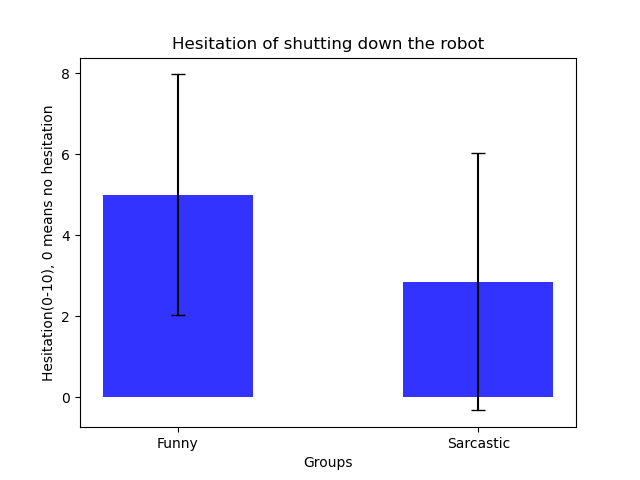
\includegraphics[width = \linewidth]{Pics/HesitationBar.png}
        \caption{Bar chart with whiskers of hesitation.}
        \label{fig:HesitationBar}
    \end{figure}
    
    \begin{table}[htbp]
        \centering
        \begin{tabular}{|l|c|c|}
        \hline
        \textbf{Anthropomorphism} & \textbf{P-value} & \textbf{Cohen's d} \\
        \hline
        \textbf{Fake-Natural} & 0.321 & 0.535 \\
        \hline
        \textbf{Machinelike-Humanlike} & 0.947 & 0.137 \\
        \hline
        \textbf{Unconscious-Conscious} & 0.495 & 0.508 \\
        \hline
        \textbf{Artificial-Lifelike} & 0.461 & 0.451 \\
        \hline
        \textbf{Rigidly-Elegantly} & 0.781 & 0.189 \\
        \hline
        \end{tabular}\\
        \vspace{5pt}
        \caption{Anthropomorphism ratings}
        \label{tab:anthropomorphism}
    \end{table}

    \begin{table}[htbp]
        \centering
        \begin{tabular}{|l|c|c|}
        \hline
        \textbf{Animacy} & \textbf{P-value} & \textbf{Cohen's d} \\
        \hline
        \textbf{Dead-Alive} & 0.946 & 0.254 \\
        \hline
        \textbf{Stagnant-Lively} & 0.638 & 0.368 \\
        \hline
        \textbf{Mechanical-Organic} & 1.0 & 0.0 \\
        \hline
        \textbf{Inert-Interactive} & 0.429 & 0.425 \\
        \hline
        \textbf{Apathetic-Responsive} & 0.523 & 0.304 \\
        \hline
        \end{tabular}
        \vspace{5pt}
        \caption{Animacy ratings}
        \label{tab:animacy}
    \end{table}
    
\begin{table}[htbp]
\centering
\begin{tabular}{|l|c|c|}
\hline
\textbf{Likeability} & \textbf{P-value} & \textbf{Cohen's d} \\
\hline
\textbf{Dislike-Like} & 0.785 & 0.293 \\
\hline
\textbf{Unfriendly-Friendly} & 0.204 & 0.741 \\
\hline
\textbf{Unkind-Kind} & 0.202 & 0.723 \\
\hline
\textbf{Unpleasant-Pleasant} & 0.789 & 0.128 \\
\hline
\textbf{Awful-Nice} & 0.943 & 0.131 \\
\hline
\end{tabular}
\vspace{5pt}
\caption{Likeability ratings}
\label{tab:likeability}
\end{table}

\FloatBarrier
    \begin{figure}[htbp]
        \centering
        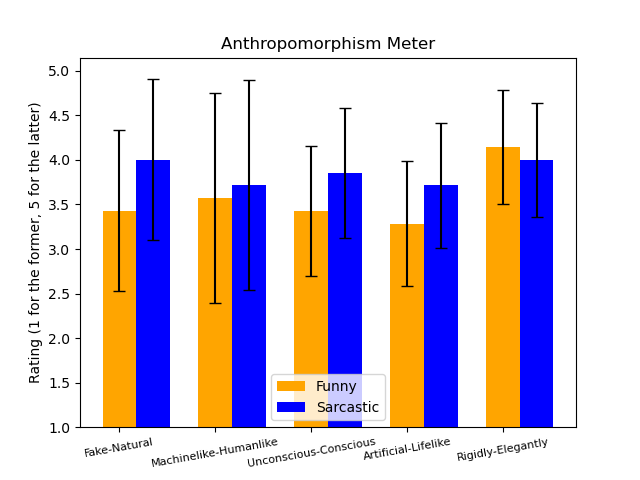
\includegraphics[width = \linewidth]{Pics/AnthroBar.png}
        \caption{Bar chart of anthropomorphism meter.}
        \label{fig:AnthroBar}
    \end{figure}

        \begin{figure}[htbp]
        \centering
        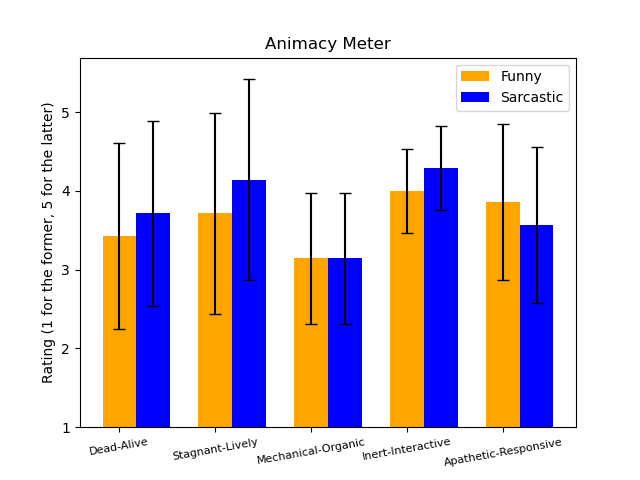
\includegraphics[width = \linewidth]{Pics/AnimacyBar.png}
        \caption{Bar chart of animacy meter.}
        \label{fig:AnimacyBar}
    \end{figure}

        \begin{figure}[htbp]
        \centering
        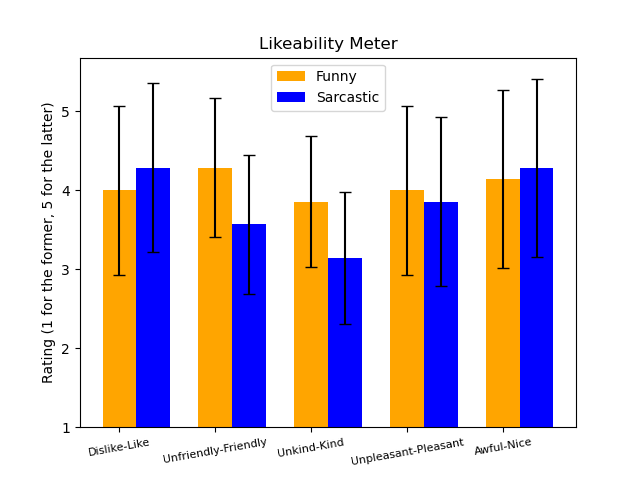
\includegraphics[width = \linewidth]{Pics/Likeability.png}
        \caption{Bar chart of likeability meter.}
        \label{fig:LikeabilityBar}
    \end{figure}


\section{Discussion}



\textcolor{red}{\textbf{THIS IS AN INDIVIDUAL PART.}}

\textcolor{blue}{
In the Discussion Section you should describe how you interpret the results of your user study. 
The goals for the Discussion Section are as follows:\\
• Critically analyse and interpret the findings of your study.\\
• Place your findings in the context of published literature. E.g., you can compare how 
your results are similar or different to results from related work.\\
• Describe how your study moves the research field forward.\\
• Describe any limitations of your study. This is a mandatory part of the Discussion 
Section.\\
• Reflect on the process of conducting your study. What went well? What went badly? 
How would you change your study design and execution to improve it? This is a 
mandatory part of the Discussion Section.
}

\section{Conclusion}

\textcolor{red}{\textbf{THIS IS AN INDIVIDUAL PART.}}

\textcolor{blue}{The conclusion rounds off your report. In the conclusion, answer the following questions:\\
• What is the main take home message of your study?\\
• What is the main contribution that your study makes to the HRI research field?\\
• For whom are the study results important? E.g., which end users could be interested 
in your results?\\
• End the conclusion with a discussion of future directions for your research. What follow 
up studies should be conducted based on your results?}



% \begin{thebibliography}{00}
% \bibitem{b1} G. Eason, B. Noble, and I. N. Sneddon, ``On certain integrals of Lipschitz-Hankel type involving products of Bessel functions,'' Phil. Trans. Roy. Soc. London, vol. A247, pp. 529--551, April 1955.
% \bibitem{b2} J. Clerk Maxwell, A Treatise on Electricity and Magnetism, 3rd ed., vol. 2. Oxford: Clarendon, 1892, pp.68--73.
% \bibitem{b3} I. S. Jacobs and C. P. Bean, ``Fine particles, thin films and exchange anisotropy,'' in Magnetism, vol. III, G. T. Rado and H. Suhl, Eds. New York: Academic, 1963, pp. 271--350.
% \bibitem{b4} K. Elissa, ``Title of paper if known,'' unpublished.
% \bibitem{b5} R. Nicole, ``Title of paper with only first word capitalized,'' J. Name Stand. Abbrev., in press.
% \bibitem{b6} Y. Yorozu, M. Hirano, K. Oka, and Y. Tagawa, ``Electron spectroscopy studies on magneto-optical media and plastic substrate interface,'' IEEE Transl. J. Magn. Japan, vol. 2, pp. 740--741, August 1987 [Digests 9th Annual Conf. Magnetics Japan, p. 301, 1982].
% \bibitem{b7} M. Young, The Technical Writer's Handbook. Mill Valley, CA: University Science, 1989.
% \end{thebibliography}
% \vspace{12pt}
% \color{red}
% IEEE conference templates contain guidance text for composing and formatting conference papers. Please ensure that all template text is removed from your conference paper prior to submission to the conference. Failure to remove the template text from your paper may result in your paper not being published.

\bibliographystyle{IEEEtran}
\bibliography{main}

\appendix

The study paperwork (participant information sheet, informed consent, ethical review) are attached at the end.




%\textcolor{red}{\textbf{THIS IS A SHARED PART.}}

%\textcolor{blue}{Please add the study paperwork (participant information sheet, informed consent, etc.) as appendix to the report.}

\onecolumn

\includepdf[pages=-]{Appendix/Information.pdf}
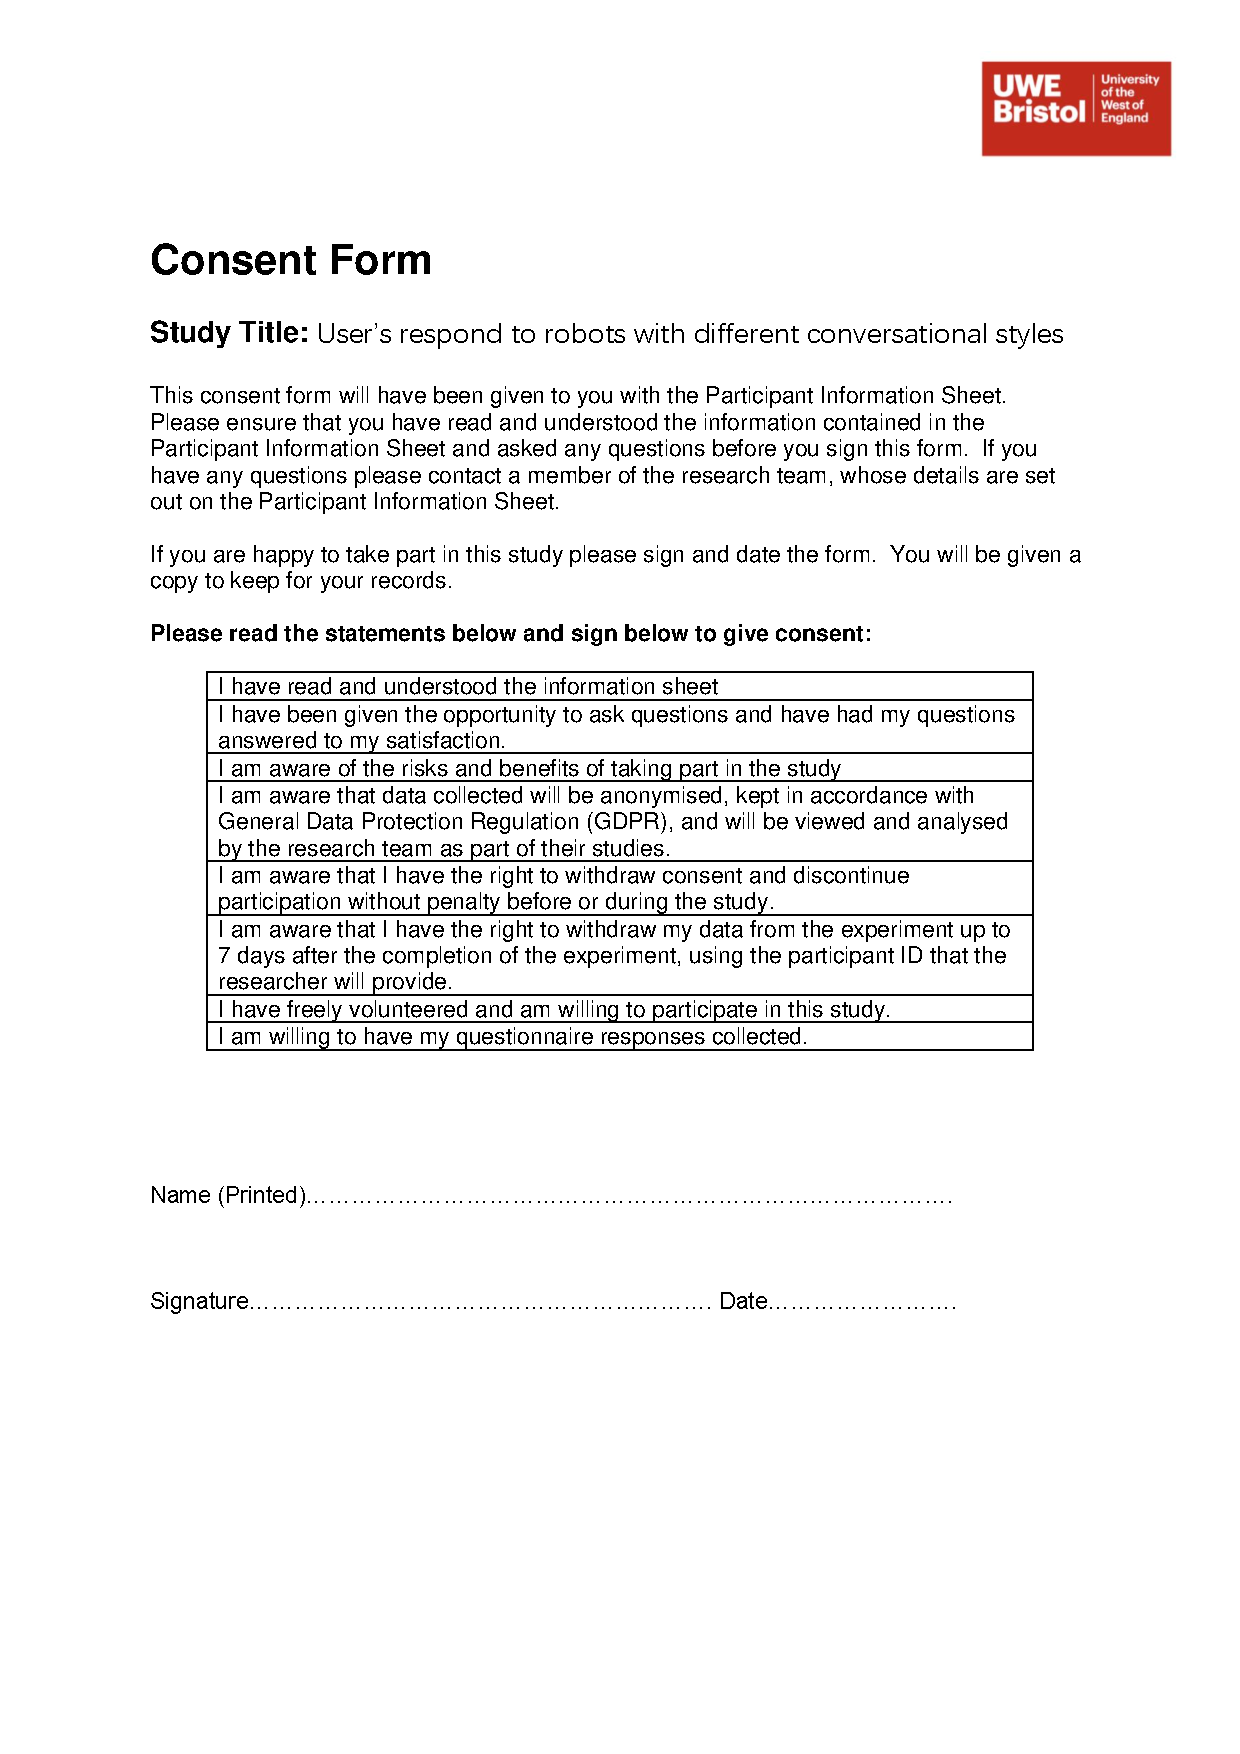
\includepdf[pages=-]{Appendix/Consent.pdf}
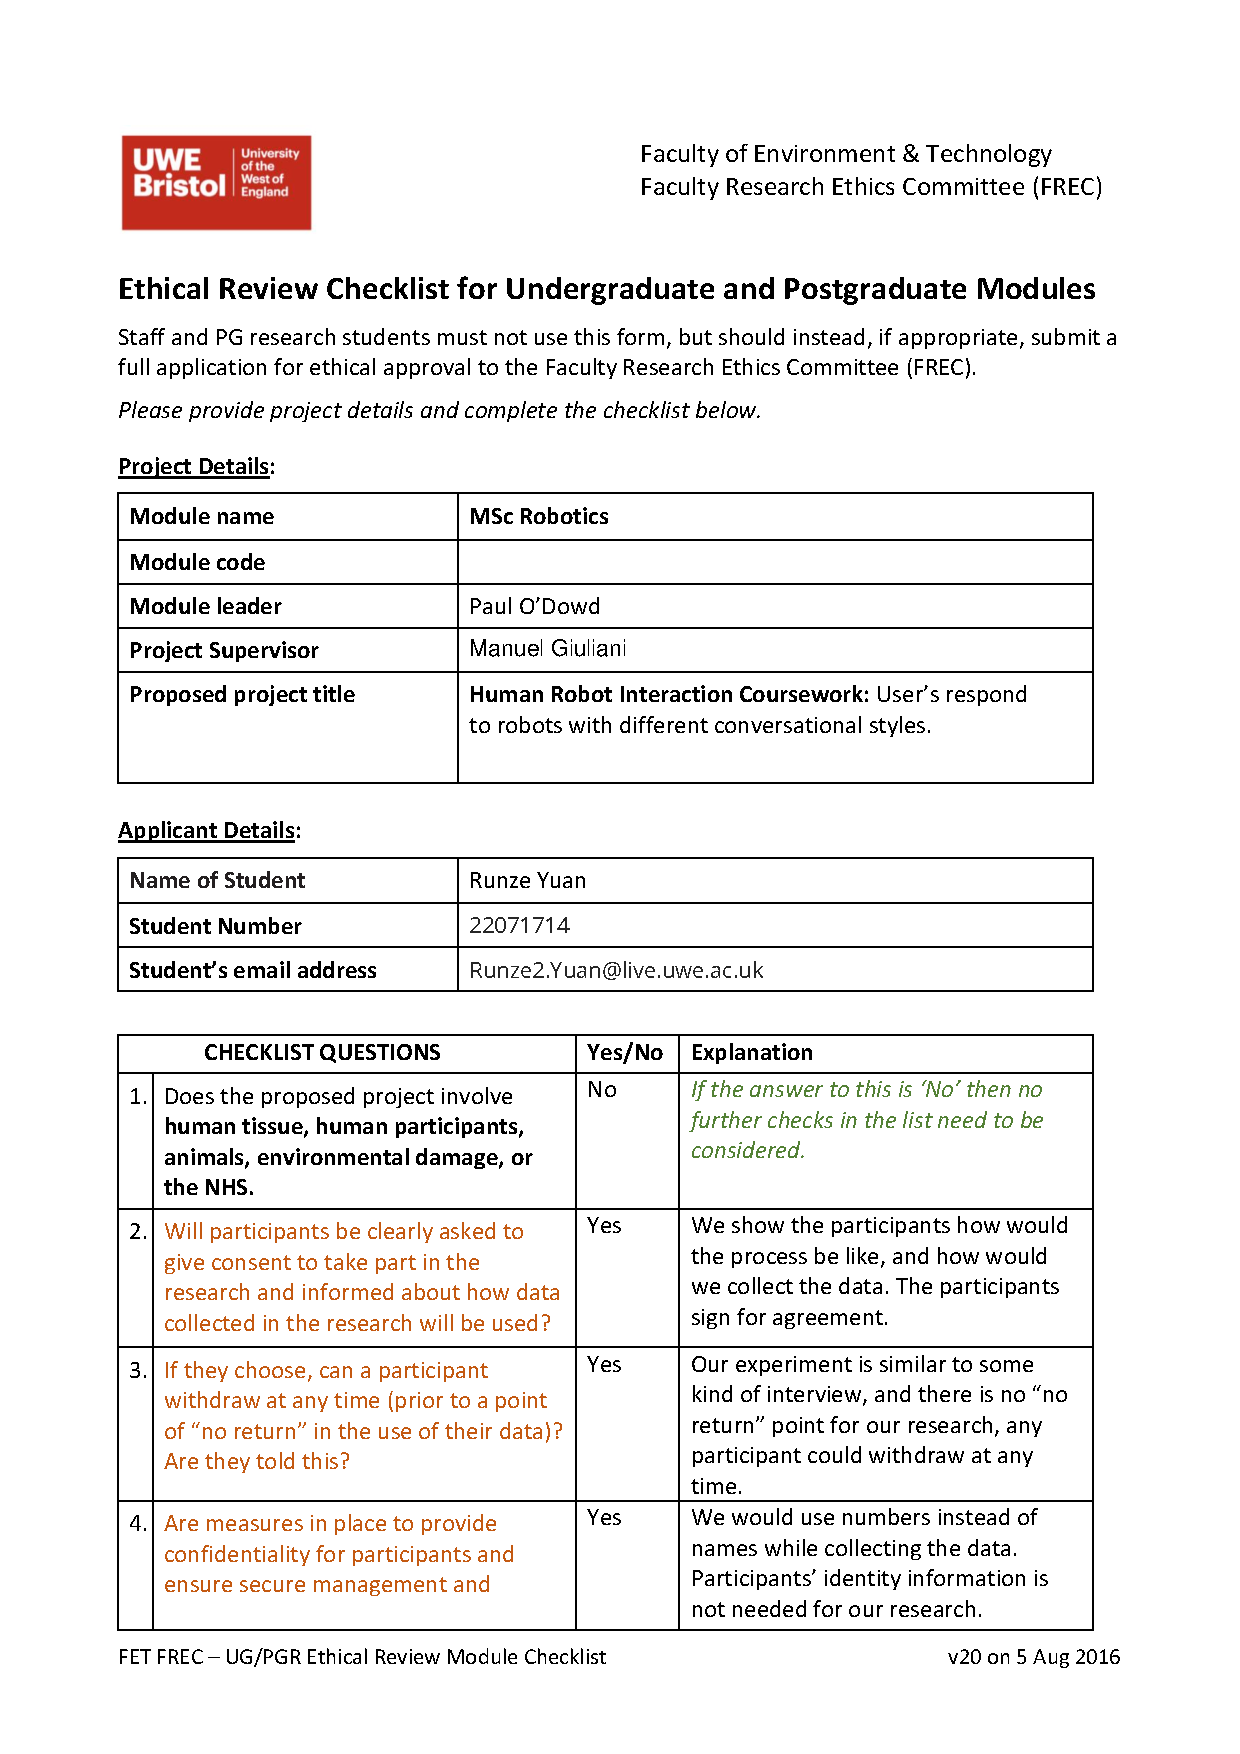
\includepdf[pages=-]{Appendix/Ethic.pdf}
\end{document}
